\documentclass[12pt,a4paper,titlepage]{book}
\usepackage[utf8]{inputenc}
\usepackage{amsmath}
\usepackage{amsfonts}
\usepackage{amssymb}
\usepackage{makeidx}
\usepackage{graphicx}
\usepackage{hyperref} % voor http links
\usepackage{listings} % om programma code te formateren
\usepackage{tikz} %% voor allerlei grafische dingen, met name flowcharts
\usetikzlibrary{shapes,arrows}

\author{Frans Schneider}
\title{pm: Een Erlang gebaseerde Policy Machine implementatie}

\begin{document}

	\maketitle
	\tableofcontents
	\listoffigures
	%% \listoftables
	\lstlistoflistings
	
	%% instellingen voor het maken van programma listings
	\lstset{
		language=erlang,
		basicstyle=\small\ttfamily,
		breaklines=true,                 % sets automatic line breaking
		captionpos=b,                    % sets the caption-position to bottom
		keepspaces=true,                 % keeps spaces in text
		tabsize=4
	}
	
	\chapter{Introduction}
	
	For an introduction to the Policy Machine (PM), access control and other related stuff, see \cite{NISTIR-7987-REV-1}, \cite{NISTIR-7316}, \cite{Assessment-AC-Systems}. Read the first two chapters of Ferraiolo et al \cite{NISTIR-7987-REV-1} and then come back for the details of the implementation.
	
	This text is shamelessly copied from \cite{NISTIR-7987-REV-1} and other material, i.e. we just took whatever fragments we needed and pasted them in this document. Since I am not a native English speaker, I have to amend the original text with examples and some remarks to understand what is written.
	
	\section{Core Policy Elements}
	
	\begin{description}
		\item[users] (U) are \emph{individuals} that have been \emph{authenticated} by the system. Users have unique identifiers within the system;
		
		\item[processes] (P) is a system entity	with memory, which \emph{operates on behalf} of a user. Users submit access requests through processes. The PM treats users and processes as independent but related entities. Processes can issue access requests, have exclusive access to their own memory, but none to that of any other process. A user may be associated with one or more processes, while a process is always associated with just one user. The function \lstinline|Process_User(p)| returns the user $u \in U$ associated with process $p \in P$. A user may create and run various processes from within a \emph{session}. The PM model permits only one session per user, however.
		$\forall p \in P, \exists _1 u \in U: u = \operatorname{Process\_User}(p)$;
		
		\item[objects] (O) are system entities that are subject to control under one or more defined policies. Objects are the actual \emph{things} under control, such as a file including its content, an e-mail message, a printer etc. It is the actual thing! Objects have unique identifiers within the system;
		
		\item[user and object attributes] (UA and OA) are policy elements that represent important characteristics, which are used to organize and distinguish respectively between classes of users and objects. The identifier of a user and object are treated not
		only as a user or an object within PM relations, but may also be treated as an user or object attribute based on its context within a relation, e.g. the name of a file is an object attribute while the file is the object. By definition, every object is considered to be an object attribute within the PM model; i.e., $O \subseteq OA$.\footnote{Why doesn't hold the same for user and user attributes?}
		
		\item[policy classes] (PC) is used to organize and distinguish between distinct types of policy being expressed and enforced. A policy class can be thought of as a container for policy elements and relationships that pertain to a specific policy. For example, there could be two policy classes---Project Access and File Management---involved in the decision process;
		
		\item[operations] (Op) denote actions that can be performed on the contents of objects that represent resources or on PM data elements and relations that represent policy. The entire set of generic operations, Op, are partitioned into two distinct, finite sets of operations: \emph{resource} operations, ROp, and \emph{administrative} operations, AOp. Common resource operations include \emph{read} and \emph{write}, for example,
		Resource operations can also be defined specifically for the environment in which the PM is implemented. Administrative operations on the other hand pertain only to the creation
		and deletion of PM data elements and relations. $Op = ROp \cup AOp$;
		
		\item[access rights] (AR) are required to be able to carry out an operation. As with
		operations, the entire set of access rights, AR, are partitioned into two distinct, finite sets of access rights: resource access rights, RAR, and administrative access rights AAR. Normally a one-to-one mapping exists between ROP and RAR, but not necessarily between AOP and AAR. For example, for the operations \emph{read} and \emph{write} the ARs \lstinline|r| and \lstinline|w| respectively are required. $AR = RAR \cup AAR$;
		
		\item[policy element] (PE) where $PE = U \cup UA \cup OA \cup PC$ and $O \subseteq OA$.
		
	\end{description}

	\section{Assignment Relation}
	
	Assignments are the means used to express relationships between users and user attributes,
	objects and object attributes, user (object) attributes and user (object) attributes, and user (object) attributes and policy classes. The assignment relation is a binary relation on the set of policy elements, PE, where $PE = U \cup UA \cup OA \cup PC$ and $O \subseteq OA$. An individual assignment can be expressed as either $(x, y) \in ASSIGN$ or $x ASSIGN y$, on elements $x$, $y$ of $PE$. The assignment relation is defined as follows:
	
	\begin{equation}
	ASSIGN \subseteq (U \times UA) \cup (UA \times UA) \cup (OA \times OA) \cup (UA \times PC) \cup (OA \times PC) 
	\end{equation}
	
	The assignment relation must satisfy the following properties:
	
	\begin{itemize}
	
		\item It is irreflexive;
		
		\item It is acyclic;
		
		\item A sequence of assignments (i.e., a path) must exist from every element in U, UA, and OA to some element in PC;
		
		\item An object attribute cannot be assigned to an object.
	
	\end{itemize}

	The assignment relation can be represented as a directed graph or digraph G = (PE, ASSIGN),
	where PE are the vertices of the graph, and each tuple $(x, y)$ of ASSIGN represents a direct edge or arc that originates at x and terminates at y.
	
	\begin{figure}[h]
		\centering
		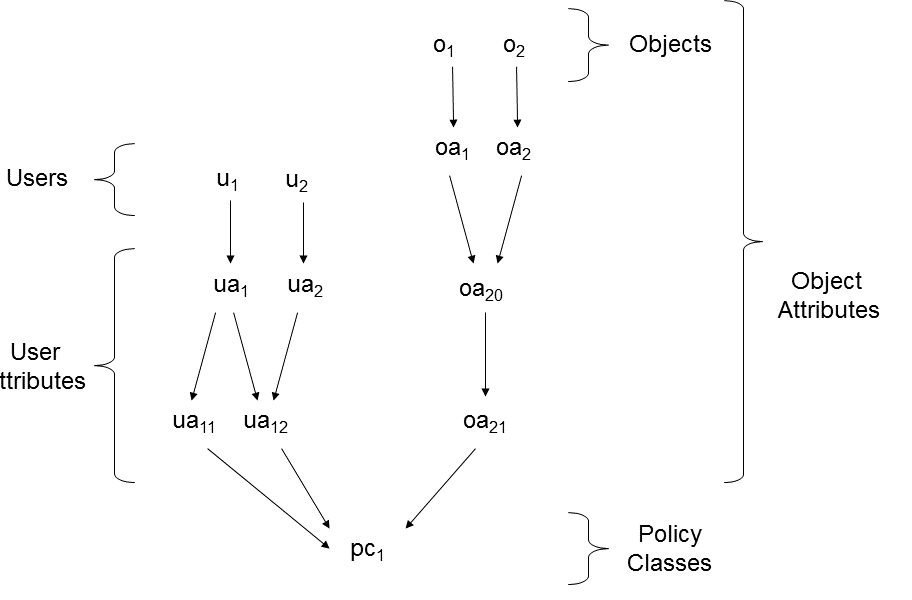
\includegraphics[width = 0.8\textwidth]{images/simplified_PE_diagram.png}
		\caption{Simplified Policy Element Diagram}
		\label{fig:simplifiedPEdiagram}
	\end{figure}
	
	The transitive closure\footnote{the concept of transitive closure can be thought of as constructing a data structure that makes it possible to answer reachability questions. That is, can one get from node a to node d in one or more hops? A binary relation tells you only that node a is connected to node b, and that node b is connected to node c, etc. After the transitive closure is constructed one may determine that node d is reachable from node a. See this Wikipedia page on transitive closure  \href{https://en.wikipedia.org/wiki/Transitive\_closure\#In\_graph\_theory}{in graph theory}} of the relation ASSIGN is written as $ASSIGN^+$. The expression $x \ 
	ASSIGN^+ \ y$ denotes that a series of assignments exists from x to y. Transitive closure is synonymous with the concept of containment. For instance, in the example in figure  \ref{fig:simplifiedPEdiagram}, the user attribute $ ua_{12} $ can be said to contain the policy elements $ u_1, u_2, ua_1, ua_2 $, while user attribute $ ua_{11} $ can be said to contain the policy elements $ u_1, ua_1 $.
	
	The reflexive and transitive closure of the relation ASSIGN, denoted as $ASSIGN^*$, is a convenient way to represent that one element in PE is contained by another through a 	series of zero or more assignments. Several helpful functions that make use of the transitive closure and the reflexive and transitive closure relations can now be defined. They are the:
	
	\begin{description}
		
		\item[Users] function from $ UA $ to $ 2^U $, which represents the mapping from a user attribute to the set of users that are contained by that user attribute. Intuitively, the function $ \operatorname{Users}(ua) $ returns the set of users that are contained by or possess the characteristics of the user attribute $ ua $. The function is defined as $ \operatorname{Users} \subseteq UA \times 2^U $;
		
		\item[Objects] function, which represents the mapping from an object attribute to the set of objects that are contained by that object attribute. Intuitively, the function $ \operatorname{Objects}(oa) $ returns the set of objects that are contained by or possess the characteristics of the object attribute $ oa $. Since all objects are, by definition, members of the set of object attributes, the function must also include the domain of the function within its range, in such instances. The Objects function is a total function from $ OA $ to $ 2*O $, which is defined as $ \operatorname{name}Objects \subseteq OA \times 2^O $;
		
		\item[Elements] function generalizes this concept for any policy element. The Elements function is a total function from $ PE $ to $ 2^{PE} $, which represents the mapping from a given policy element to the set of policy elements that includes the policy element and all the policy elements contained by that policy element. The function is defined as $ \operatorname{Elements} \subseteq PE \times 2^{PE} $.
		
	\end{description}
	
	\subsection{User and Object Assignments}
	
		A user may be assigned to one or more user attributes. The assignment $ u ASSIGN ua $ means that the user u is assigned to or contained by the user attribute ua. It also denotes that user u takes on or acquires the properties held or represented by the attribute ua. The properties of a user attribute are defined as the capabilities for and constraints against accessing certain types of objects.
		
		Similarly, an object may be assigned to one or more object attributes through one or more object-to-attribute assignments, represented as a binary relation from O to OA. The assignment $ o ASSIGN oa $ means that that the object o is assigned to or contained by the object attribute oa and takes on or acquires the properties held by the attribute oa. The properties of an object attribute are defined as the capabilities and constraints allotted to users, which govern access to contained objects (i.e., the access modes allowed and denied to specific users).
		
	\subsection{Attribute Assignments}
	
		A user (object) attribute may be assigned to one or more other user (object) attributes.
		Assignments between user (object) attributes are, by definition, restricted to attributes of the same type (i.e., either all user attributes or object attributes). Containment, as it applies to assignments among attributes, denotes that a user (object) attribute takes on or acquires the properties held or represented by each user (object) attribute that contains it. Containment allows each attribute to augment the properties conferred directly to it with the properties held by every attribute that contains it.
		
		Assignments among attributes have an effect on the way users and objects contained by those
		attributes are treated within the PM model. A user x that is contained by user attribute y gains the properties that are both assigned to and acquired by attribute y. Similarly, an object x that is contained by object attribute y, gains the properties that are both assigned to and acquired by attribute y.
		
	\subsection{Policy Class Assignments}
	
		A user attribute or an object attribute may be assigned to one or more policy classes. As
		mentioned earlier, a policy class can be thought of as a container for policy elements and
		relationships that pertain to a specific policy; every policy element is contained by at least one policy class. Unlike attributes, however, a policy class cannot be assigned to any other policy class. In addition, since policy classes do not have properties associated with them, attributes assigned to a policy class do not acquire any properties from it.
		
		Policies can be constructed\footnote{How??} such that policy elements of one policy class are defined to be mutually exclusive from those of another policy class. That is, if a policy element $ x $ is contained by $ pc_1 $ in such a policy, it would be precluded from being contained by $ pc_2 $ or some other policy class. Policy elements can also be defined to be inclusive of more than one policy class.
		
		An access control policy can be characterized through a single policy class, multiple mutually exclusive policy classes, or multiple non-mutually exclusive policy classes.
		
	\section{Associations and Privilege Relations}
	
	Associations define relationships that represent the authorization of access rights between policy elements. Privileges are derived from association and assignment relations andare shaped in part by the attribute to attribute assignments defined for a policy.
	
	\subsection{Associations}
	
		The association relation is a policy setting that governs which users are authorized to access which objects and exercise which access rights. For each policy class containing attribute at, the association ua—ars—at specifies that all users contained by ua possess the authority denoted by ars over at and all policy elements contained by at.
		
		Note that attributes appearing within a relation, such as the association relation, often serve as referents. A referent attribute is treated as a designator or representative for the policy elements it contains and possibly the attribute itself, depending on the semantics of the relation. Each referent represents a policy graph containing all policy elements from which the referent is reachable through one or more assignments, and affects all relationships bound to those elements.
		
		Within the context of an association, (ua, ars, at), the third term, attribute at, is treated as a referent for the policy elements within the section of the policy element diagram rooted at the attribute, as well as itself. Similarly, the first term, attribute ua, is treated as a referent for the users and user attributes within the section of the policy element diagram rooted at ua. Although a referent potentially represents many policy elements and relationships, an access right may be pertinent to only a subset of the policy elements that are represented by the referent. That is, an access right might be relevant for one or more of the policy elements a referent attribute contains, or the access right might have relevance only to the attribute itself—it depends entirely on the access right. For example, an association involving r and w access rights on an object attribute are relevant for the objects contained by the attribute, but not for the attribute or contained attributes.
		
		Although not mandatory, as a rule of practice, specifying associations that involve resource
		access rights separately from associations that involve administrative access rights is advised. One reason for segregating associations this way is that a different perspective applies to each type. Resource associations do not authorize changes to policy and are directed mainly at the actions of ordinary users, while administrative associations are more complex, since they allow policy alterations to occur, and are directed mainly at policy authorities. Another difference relates to access requests: each resource operation is synonymous with and authorizable via a single resource access right (e.g., a “read” operation requires an “r” access right), authorization for an administrative operation, however, often requires possession of multiple administrative access rights.
	
	\subsection{Containment and Attribute Properties}
	
		Assignments among attributes affect the interpretation of associations. As mentioned earlier, the inherent properties of an attribute include not only those conferred directly to the attribute, but also the properties it acquires from every attribute in which it is contained. A simple example to demonstrate containment among attributes is given in Figure \ref{fig:SimpleAuthorizationGraph}.
		
		\begin{figure}[h]
			\centering
			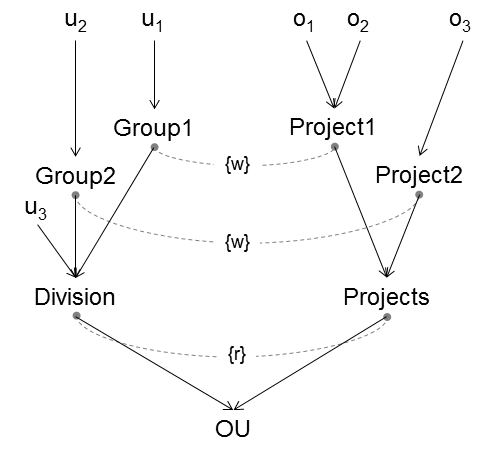
\includegraphics[width = 0.8\textwidth]{images/simple_authorization_graph.png}
			\caption{Simple Authorization Graph}
			\label{fig:SimpleAuthorizationGraph}
		\end{figure}
		
		Associations are illustrated using dotted, downward-arcing connectors between the elements involved in each association. The inherent properties of each user attribute in the diagram can be determined, by combining those properties granted directly to the attribute through a defined association with those acquired indirectly through containment by an attribute possessing the property. In \cite{NISTIR-7987-REV-1} \S 3.3.2 (p20) gives a detailed description of the properties derived from the example in figure \ref{fig:SimpleAuthorizationGraph}.
		
		\subsection{Derived Privileges}
		
		A privilege specifies a relationship between a user, an access right, and an attribute. Privileges are derived from higher level relations, namely the associations between and the assignments among attributes. That is, every privilege originates from an association and the containment properties of the user attribute and the target attribute of that association, which are designated through assignments.
		
		The ternary relation $ PRIVILEGE \subseteq U \times AR \times (PE \setminus PC) $ defines the set of possible privileges within a policy specification. An individual tuple of PRIVILEGE, $ (u, ar, e) $, denotes that user u holds the authority to exercise the access right ar on policy element e. The privilege relation may be partitioned into two parts, $ PRIVILEGE \subseteq (U \times RAR \times (PE \setminus PC)) \cup (U \times AAR \times (PE \setminus PC))$ for resource and administrative related privileges.
		
	\section{Prohibitions and Restriction Relations}

	Prohibitions define relationships that govern the suppression of access rights between policy
	elements. Three distinct, but related types of prohibitions exist: user-based, process-based, and user attribute-based prohibitions. Prohibitions in a way can be thought of as the antithesis of associations, because restrictions, which are derived from prohibitions, essentially negate privileges that would otherwise allow access to occur. That is, each type of prohibition denotes an effective set of restrictions, which represent privileges that a specific user, process, or class of users is precluded from exercising, regardless of whether the user, process, or class of users in question hold any of the actual privileges.
	
	\begin{figure}[h]
		\centering
		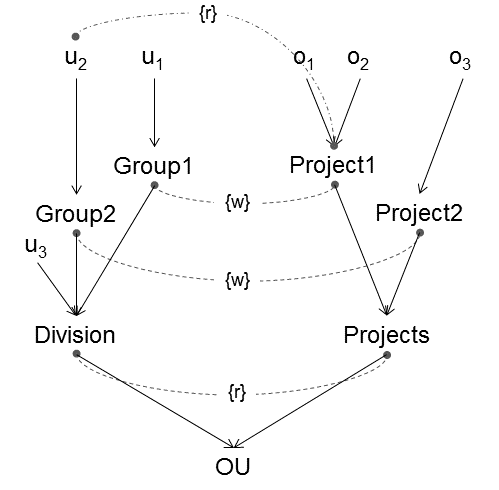
\includegraphics[width = 0.8\textwidth]{images/Authorization_Graph_with_Prohibition.png}
		\caption{Authorization Graph with Prohibition}
		\label{fig:AuthorizationGraphWithProhibition}
	\end{figure}

	To illustrate the use of prohibitions, Figure \ref{fig:AuthorizationGraphWithProhibition} re-illustrates the example authorization graph discussed the previous section, augmented with a single user prohibition. The prohibition is depicted using a dotted, upward-arcing connector.
	
	The set of policy elements affected by a prohibition is designated via either conjunctive or disjunctive mappings over sets of referent attributes to the policy elements in question. A pair of functions facilitate the discussion of the affected policy elements. 
	
	The disjunctive range function represents the mapping from two constraint sets of attributes—the first designating policy elements for inclusion, and the second designating policy elements for exclusion—to a set of policy elements formed by logical disjunction of the policy elements contained within or not contained respectively within the subgraphs of the referent attributes of each constraint set. 
	
	Similarly, the conjunctive range function represents the mapping from two constraint sets of attributes—the first designating policy elements for inclusion, and the second designating policy elements for exclusion—to a set of policy elements formed by logical conjunction of the policy elements contained by or not contained by the attributes of each constraint set respectively.
	
	The following types of prohibitions exist:
	
	\begin{itemize}
		\item User-based Prohibitions and Restrictions] description;
		\item Process-based Prohibitions and Restrictions and
		\item Attribute-based Prohibitions and Restrictions.
	\end{itemize}		
		
	\section{Obligations}
	
	Obligations represent potential changes to the authorization state of the policy. They are used when one or more administrative actions need to be carried out under a specific, known set of circumstances. Events are the means by which obligations are triggered. An event occurs each time a requested access executes successfully. Information related to the event is called the event context and is used by the PM to process obligations. The process identifier, identifier of the associated user, access operation, and sequence of arguments of the triggering event are mandatory and always returned as part of the event context.
	
	The two main components needed to define an obligation are an event pattern and a response. The pattern and response elements each denote a sentence in a grammar that respectively expresses the triggering conditions of an event pattern and the administrative actions of the response. The event pattern and response each represents sentences that must conform to a formal language over their respective alphabet.
	
	The obligation relation, OBLIG, is defined as a ternary relation from U to PATTERN to RESPONSE. For each tuple (u, pattern, response) of the obligation relation, u represents the user that established the pattern and response, and under whose authorization the response is carried out. The pattern and response of obligation is sometimes expressed like \lstinline|when <pattern> do <response>|.
	
	\section{Access Request Decisions}
	
	Authenticated users do not generate access requests directly, but instead instantiate one or more processes to generate requests on their behalf. The access decision function controls accesses in terms of processes. The user on whose behalf the process operates must hold sufficient authority over the policy elements involved in the request, in the form of at least one and possibly several privileges. That is, an access request to perform an operation on a policy element, including objects, are issued only from processes acting on behalf of some user, and is granted provided the appropriate privileges exist that allow the access, and no restriction exists that prevents the access. If a restriction does exist, the access request is denied.
	
	The relation, $ AREQ \subseteq P \times Op \times Argseq $ defines the set of access requests. A tuple of the access request relation, (p, op, argseq), denotes that process, p, is requesting to perform the operation, op, on the resource or policy items referenced by the argument sequence, argseq. The argument sequence is a finite sequence of one or more arguments, which is compatible with the scope of the operation. Each argument in the sequence can be either a distinct policy element, a set of policy elements, a set of access rights, an event pattern, or an event response, as is appropriate for the operation. That is, an access request comprises an operation and a list of enumerated arguments whose type and order are dictated by the operation. Note that resource operations typically take an argument sequence comprising a single element (viz., an object identifier), while administrative operations typically take an argument sequence comprising multiple elements.
	
	The access decision function grants a process, p, permission to execute an access request (p, op, argseq), provided the following conditions hold for each access right and policy element pair (ar, pe) in one of the capability sets returned by the required capabilities function, ReqCap(op, argseq):
	
	\begin{itemize}
		
		\item There exists a privilege $ (Process_User(p), ar, pe) $;
		
		\item There does not exist a process restriction $ (p, ar, pe) \in P\_RESTRICT $;
		
		\item There does not exist a user restriction $ (Process\_User(p), ar, pe) \in U\_RESTRICT $;
		
		\item There does not exist a user attribute restriction $ (ua, ar, pe) \in UA\_RESTRICT $, such that Process\_User(p) is contained by user attribute ua.
		
	\end{itemize}
	
	Otherwise, the requested access is denied.
	
	\begin{figure}[h]
		\centering
		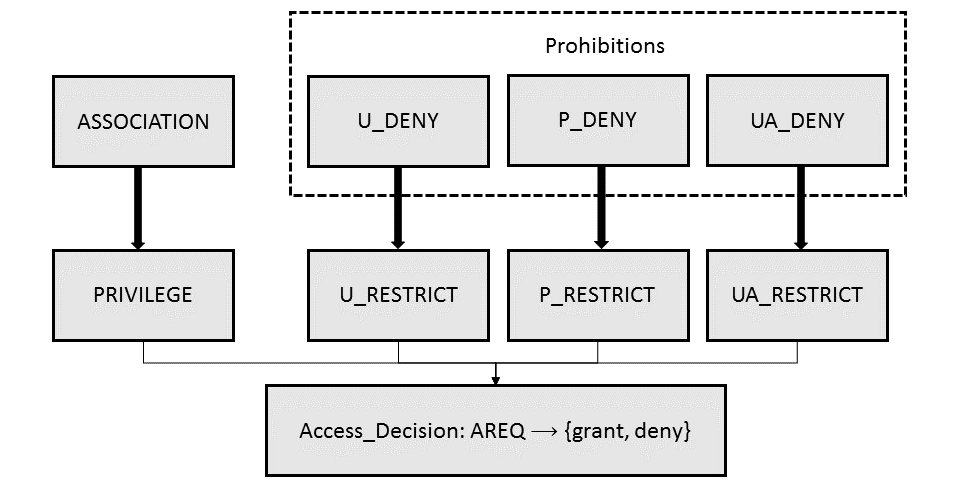
\includegraphics[width = 0.8\textwidth]{images/ComputingAccessDecision.png}
		\caption{Computing an Access Decision}
		\label{fig:ComputingAccessDecision}
	\end{figure}
	
	\chapter{Other Considerations}
	
	\section{Administrative Commands and Routines}
	
	\begin{figure}[h]
		\centering
		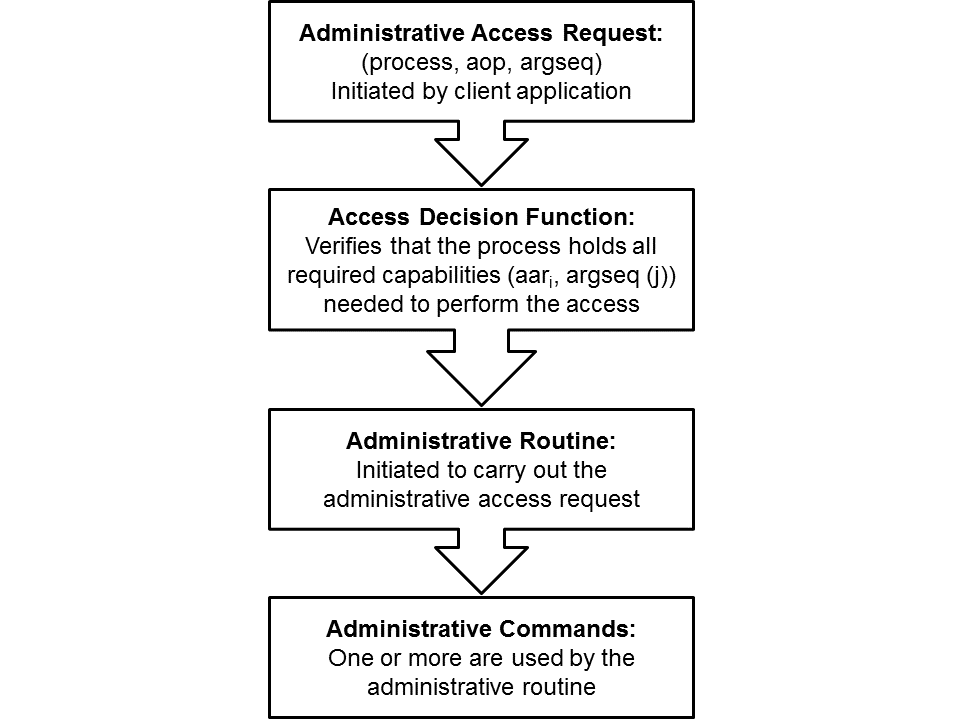
\includegraphics[width = 0.8\textwidth]{images/AdministrativeRoutinesCommandsAccessRequestProcessing.png}
		\caption{Administrative Routines and Commands in Access Request Processing}
		\label{fig:AdministrativeRoutinesCommandsAccessRequestProcessing}
	\end{figure}
	
	\begin{description}
		
		\item[Administrative commands] describe rudimentary operations that alter the policy elements and relationships of the PM model, which comprise the authorization state. An administrative command is represented as a parameterized procedure, whose body describes state changes to policy that occur when the described behavior is carried out (e.g., a policy element or relation Y changes state to Y' when some function f is applied). Administrative commands are specified using the following format:
		\begin{lstlisting}
Cmdname(x1 : type1, x2 : type2, ..., xk : typek)
  ... preconditions ...
  {
    Y` = f(Y, x1, x2, ..., xk)
  }\end{lstlisting}
		
		\item[Administrative routines] consist mainly of a parameterized interface and a  sequence of  administrative command invocations. Administrative routines build upon administrative commands to define the protection capabilities of the PM model. The body of an administrative routine is executed as an atomic transaction—an error or lack of capabilities that causes any of the constituent commands to fail execution causes the entire routine to fail, producing the same effect as though none of the commands were ever executed. Administrative routines are specified using the following format:
		\begin{lstlisting}
Rtnname(x1 : type1, x2 : type2, ..., xk : typek)
  ... preconditions ...
  {
    cmd1 ;
    condition a cmd2, cmd3;
    . . .
    condition z cmdn;
  }\end{lstlisting}

	\end{description}

	First and foremost, administrative routines are used to define services of the PM model. An administrative routine must be in place to carry out each valid administrative access request of the PM model on a one-to-one basis. The PM model routines form the trusted computing base of the PM framework. Another common use of administrative routines is in the definition of an obligation, as the response to be taken whenever the corresponding event pattern is matched. Administrative routines can also be used to facilitate the administration of system policies.
	
	\section{Multiple Policy Class Considerations}
	
	Some policy specifications can involve more than one policy class. Multiple policy class situations may arise when two or more policies, each represented by a single policy class, are brought together and overlap to the extent that some policy elements fall under each policy. They can also occur when an administrator chooses to express a single policy using multiple policy classes, even though the policy could be expressed using a single policy class.
	
	\chapter{Implementation}
	
	\begin{figure}[h]
		\centering
		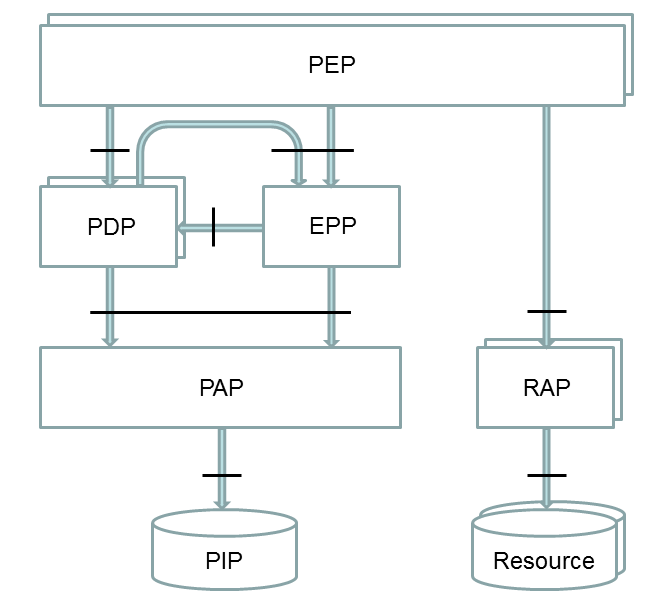
\includegraphics[width = 0.8\textwidth]{images/ArchitecturalComponentsPM.png}
		\caption{Architectural Components of the PM}
		\label{fig:ArchitecturalComponentsPM}
	\end{figure}
	
	\begin{description}
		
		\item[Policy Enforcement Point] PM-aware applications must rely on a PEP to gain access to protected resources and to policy information via the interface that it provides, which is typically a programming interface. More than one PEP may exist to service applications. The PEP ensures that access requests are verified as being in conformance with the specified policy, before the accesses in question can proceed. To accomplish this objective, the PEP works in tandem with a PDP and must not be by-passable.
		
		\item[Policy Decision Point] A PDP determines whether an access request made by a PEP complies with policy and renders a grant, deny, or error decision accordingly. The PDP performs the access decision function defined in the PM model. It also carries out all access requests that involve administrative operations for which a grant decision has been rendered. Multiple PDPs may exist in the PM environment.
		
		\item[Policy Information Point] The PIP contains the data structures that define the policy elements and the relationships between policy elements that collectively constitute the access control policy enforced by the PM. Conceptually, the PIP embodies a reification of the administrative commands.
		
		\item[Resource Access Point] A RAP allows one or more PEPs to gain access to protected resources. The only method of accessing protected resources is via a RAP. Multiple RAPs can exist, but each protected resource is accessible only through a single RAP. The PEP issues a command containing its identifier, the location of the physical resource, the operation, and any required data to the RAP. The RAP returns data and status information to the PEP. The RAP does not allow access to resources to any component other than a PEP.

		\item[Policy Administration Point] A single PAP manages all access to the contents of the PIP, similar to the way a RAP serves as a managed access point to protected resources. A PAP provides read, modify, and write access to the content within the PIP (i.e., the policy configuration). A PAP limits the EPP to read access only, but allows a PDP both read and write access.
		
		\item[Event Processing Point] A single EPP is responsible for comparing events against event patterns that have been defined in obligations residing at the PIP. For each event pattern that is matched with an event, the EPP uses a PDP to make an access request decision on the associated event response (i.e., the sequence of administrative actions defined for each obligation), and to carry out the response if the definer of the obligation holds sufficient authorization. The EPP can be viewed as a transaction processing monitor, whose performance is crucial to the overall effectiveness of the architecture.
		
	\end{description}

	\section{Handling failures}
	
	The PAP makes changes to the PIP using a set of routines based on the PIP's command set. The routines are implemented as transactions. The PIP manipulates the pm's digraph and the database. If a PAP routine fails, the database is rolled-back to the previous state, i.e. the state before the routine was executed, but the digraph can be in an inconsistent state. On failure of a PAP routine, the digraph MUST be rebuild.
	
	The commands in the PIP may fail because some condition is not met or a resource limit is exceeded. Failures in the PIP will raise Erlang errors which are handled by the PAP in the transaction as described.

	\section{Policy Information Point}
	
	The data structures used by the PIP are:
	
	\begin{description}

		\item[A digraph G] which implements the acyclic digraph the PM uses. Currently, a single digraph is used but this is likely to change because PCs may be implemented as separate digraphs;
		
		\item[A database] currently implemented using Mnesia, which stores all elements and sets the PM relies on.
		
	\end{description}
	
	The digraph G is constructed from the data in the Mnesia database on start-up of the PM. The database is implemented as a transactional store which ensures the information it holds is reliable. The digraph G however is not implemented as a transactional store which can result in it being inconsistent. Changes made in the PM by the PAP are implemented as transactions on the Mnesia database that may fail in which case the diagrah G has to be rebuild from the database. Using several smaller digraphs instead of the currently used single large digraph can reduce the effort to rebuild the digraph on a failed transaction enormously.
	Another reason to implement the digraph in separate digraphs is to reduce the use of memory resources since the digraph os kept in memory. Also think about distribution of the diagraph over nodes.
	
	The PIP implements the administrative commands listed in appendix C in \cite{NISTIR-7987-REV-1}. Quite a few of these commands are very similar to each other except for the (additional) sets they operate on, e.g. \lstinline|CreateUinUA(x:ID, y:ID)| and \lstinline|CreateUAinUA(x:ID, y:ID)| both create some X in a Y.
	The PIP has functions \lstinline|create_x(G, X)|, \lstinline|create_x_in_y(G, X, Y)| and \lstinline|delete_x(G, X)|,  which implement the basic functionality, used by the specialized functions \lstinline|create_u_in_ua| etc.
	
	By using the generic function \lstinline|create_x_in_y|, the administrative commands can defined by the PIP can also be called by the PAP without being concerned about the additional data in the different elements. The PIP only deals with the digraph related stuff while the PAP deals with the actual data, the GUIDs being part of them. For example, adding a user through the PAP involves generating the new id and adding the user name, and other data to s U element. The PIP only deals with adding the user's fresh id to the digraph.
	
	In the specs, adding an element involves the U, UA O etc. in the PIP. In this implementation, the U, UA O etc. are added to the database in the PAP with the pm relevant parts being added using the PIP. For example, in the PAP the function \lstinline|c_u_in_ua| does the following:
	
	\begin{lstlisting}[caption={Administrative routine c\_u\_in\_ua/2}]
c_u_in_ua(#u{} = U, #ua{id = Y}) ->
    ...
    X = pm_pip:allocate_id(),
    pm_pip:create_x_in_y(G, X, Y),
    mnesia:write(U#u{id = X}),
    ...\end{lstlisting}
	
	For the user a new id is generated which is assigned to X. The PIP is called to add the assignment X to Y, with Y holding the id of the UA, after which the U record is saved to the database along with the data the U record already holds, e.g. the user name.
		
	The administrative functions as defined in appendix C, all include extensive error checking on elements passed in as argument on being a member or not being e member of a particular set. In the implementation, these checks are omitted because the implementation does guaranty that every newly created element X is always unique and the functions always fail if an element Y does not already exist.	\footnote{Currently, the existence of element Y is checked by examining the set PE. If Y is not found, the function fails which will make the enclosing transaction fail. This check does not check for Y to belong to a particular set, e.g. Y belonging to UA. Is this a problem?}
	
	\subsection{create\_x\_in\_y}
	
		The \lstinline|create_x_in_y(G, X, Y)| functions takes a digraph G and adds element X to element Y.
		
		\begin{lstlisting}[caption={create\_x\_in\_y/3}, basicstyle=\footnotesize, breaklines=false, numbers=left]
-spec create_x_in_y(G :: digraph:graph(),
                    X :: pm:id(),
                    Y :: pm:id()) ->
          ok | no_return().
create_x_in_y(G, X, Y) ->
  [#pe{vertex = Vy} = PEY] = mnesia:read(pe, Y, write),
  case digraph:add_vertex(G) of
    {error, Reason} ->
      erlang:error(Reason);
    Vx ->
      case digraph:add_edge(G, Vx, Vy, Y) of
        {error, Reason} ->
          erlang:error(Reason);
        Edge ->
          %% ref_cnt for X is 1 because of the assignment
          mnesia:write(#pe{id = X, vertex = Vx, ref_cnt = 1}),
          mnesia:write(PEY#pe{ref_cnt = PEY#pe.ref_cnt + 1}),
          mnesia:write(#assign{a = X, b = Y, edge = Edge})
      end
  end. \end{lstlisting}		
	
		X is a new element, identified by its GUID. In the specs, the check $ X \notin GUID $ is made, but since this implementation guarantees that each and every new GUID is always unique, the check is omitted.
	
		Also in the specs, the check is made that X is not yet defined for the set it is added to, e.g. if X is U(ser), the check is made that X is not yet part of U. This guard is also omitted because every new element always has a unique id as described in the previously and therefor X cannot exist in the set.
		
		It is the responsibility of the calling function not to pass-in an already existing X but always first allocate a new id before calling the create functions.
		
		The next guard in the specs always is to check for Y being a member of a particular set, e.g. $ Y \in UA $, $ Y \in OA $ etc. Because we assume the functions calling this function are correct, a guard as this will always return true and has no added value and can therefor be omitted. This function is never called directly by some user code and because of that no errors can be made. Actually, the previous statement is not entirely true, because the match statement in line 6 does make sure Y exists. The match fails if $ Y \notin PE $. Line 6 matches the vertex belonging to Y to Vy and also the whole PE record to PEY for later use.
		
		A vertex for X is added to the digraph in line 7, which may fail if the system runs out of resources in which case an error is raised. If the vertex for X is created successfully, an edge is created in line 11, emanating from Vx and incident on Vy and is labeled with Y's id, which may fail in which case an error is raised. X, including the vertex belonging to it, is added to the database as a policy element (PE) with the initial reference count set to one. The database is updated for the PE Y with its reference count incremented by one. Last, the database is updated for the ASSIGN set with a set to X, b set to Y and a reference to the newly created edge.
		
		The values for the vertexes and edges in the database are used to address the current digraph directly without the need for searching. The moment the digraph becomes inconsistent, after a transaction fails, the digraph must be rebuild from the PE and assignment entries in the database, with the recalculated vertexes and edges.
		
	\subsection{delete\_u/2 and similar functions}
	
		The functions for deleting a user, user attribute, object or object attribute all look very similar:
		
		\begin{lstlisting}[caption={delete\_u/2}, basicstyle=\footnotesize, breaklines=false, numbers=left]
-spec delete_u(G :: digraph:graph(), X :: pm:id()) -> ok | no_return().
delete_u(G, X) ->
    [#u{}] = mnesia:read(u, X, write),
    delete_x(G, X),
    mnesia:delete({u, X}). \end{lstlisting}
	
		Each of these functions start by fetching the record from the database and matching it to its record type. If the policy element does not exist, this will raise an error which will abort the enclosing transaction. Next, the digraph is updated and the element is actually removed from the database.
		
		\begin{lstlisting}[caption={delete\_x/2}, basicstyle=\footnotesize, breaklines=false, numbers=left]
delete_x(G, X) ->
    %% ref_cnt must be zero for this action!  
    [#pe{vertex = V, ref_cnt = 0} = PE] = mnesia:read(pe, X, write),
    digraph:del_vertex(G, V),
    mnesia:delete_object(PE). \end{lstlisting}
    
	    A policy element can only be deleted if there are no other elements referring to it. The match in line 3 will make the function fail if the reference count is not 0. Deleting the vertex from the digraph will also delete edges emanating from V or incident on V.

	\subsection{create\_arset/2 and delete\_atset/2}\label{create_ar_atset}
	
		This function creates a access rights set, i.e. a set with one or more access rights. It takes two arguments, the id of the set and a list with access rights and stores a representation of it in the database.
		
		The same ARset can used many times all over the PM, e.g. the set {r,w} or just {r} or {w} etc. is probably used in many associations. Instead of creating a new set for each occurrence, a set can be \emph{instantiated} (used) many times.  A set is defined as a tuple with the fields \lstinline|id| for the set's id, \lstinline|value| for the set's actual set of elements, a \lstinline|ref_cnt|  to keep track of the number of times the set is referred to and an \lstinline|inst_cnt| which is equal to the number of instances of the set. The set is also referred from many places and therefor reference counted. The implementation is as follows:
		
		\begin{lstlisting}[caption={create\_arset/2}, basicstyle=\footnotesize, breaklines=false, numbers=left]
-spec create_arset(ARset :: pm:id(),
                   AR_ids :: nonempty_list(pm:id())) -> ok | no_return().
create_arset(ARset, AR_ids) ->
  case mnesia:read(arset, ARset, read) of
    [] ->
        [begin 
           [AR] = mnesia:read(ar, AR_id, write),
           mnesia:write(AR#ar{ref_cnt = AR#ar.ref_cnt + 1})
         end || AR_id <- AR_ids],
      Set = #set{id = ARset, value = sets:from_list(AR_ids),
                 ref_cnt = 0, inst_cnt = 1},
      mnesia:write(arset, Set, write);
    [#set{inst_cnt = N} = Set] ->
      mnesia:write(arset, Set#set{inst_cnt = N + 1}, write)
  end. \end{lstlisting}
	
		If a set with id \lstinline|ARset| does not exist yet (line 5), an Erlang set is created for all access rights \lstinline|AR| in the list \lstinline|AR_ids| the \lstinline|ref_cnt| is incremented because the set will reference these access rights. The list AR\_ids must not contain duplicates or the ref\_cnts will not be correct anymore. ARs with a \lstinline|ref_cnt| not being 0 can not be deleted. The actual set of access rights is constructed using the standard Erlang set and is being assigned to the value field. 
		
		If the set does already exist with the id \lstinline|ARset|, its instance count is incremented instead.
		
		The two functions delete\_arset and delete\_atset are very much identical except for the database tables used. One might consider to generalize the creation of sets and merge the two functions.
		
	\subsection{allocate\_id(Values)}
	
		The function \lstinline|allocate_id(Values)| is used to create a id based on a list of values. This function is used for example in the two functions described in \ref{create_ar_atset}. For example, to create an ARset with the two access rights \lstinline|r| and \lstinline|w|, one would use the function call \lstinline|allocate_id([r, w])| to create the new id.  Subsequent calls to the function with the same list will yield the same id. NB: order of the lists elements does make a difference for the generated id, i.e. \lstinline|[a, b]| is \emph{not} the same as \lstinline|[b, a]|.
		
	\subsection{create\_assign/3}
	
		This functions creates an assignment both in the digraph and in the database. Its implementation is the following:
		
		\begin{lstlisting}[caption={create\_assign/3}, basicstyle=\footnotesize, breaklines=false, numbers=left]
-spec create_assign(G :: digraph:graph(), X :: pm:id(), Y :: pm:id()) -> ok | no_return().
create_assign(G, X, Y) ->
  [#pe{vertex = Vx} = PEX] = mnesia:read(pe, X, write),
  [#pe{vertex = Vy} = PEY] = mnesia:read(pe, Y, write),
  case digraph:add_edge(G, Vx, Vy, Y) of
    {error, Reason} ->
      erlang:error(Reason);
    Edge ->
      mnesia:write(PEX#pe{ref_cnt = PEX#pe.ref_cnt + 1}),
      mnesia:write(PEY#pe{ref_cnt = PEY#pe.ref_cnt + 1}),
      mnesia:write(#assign{a = X, b = Y, edge = Edge})
  end.\end{lstlisting}
  
		  The arguments X and Y are the id's of the policy elements involved in the assignment. The function starts with fetching the two PEs belonging to X and Y, which in case X and Y are not existing id's will result in a failure that will abort the transaction. Next, an edge is added to the digraph between the two vertices belonging to the two PEs. Both the reference count of the two PEs are incremented and the ASSIGN set is updated in the database.
		  
	\subsection{create\_assoc/3}
	
		The \lstinline|create_assoc/3| function adds an association as a tuple \lstinline|(ua, ars, at)| to the database. An association is not part of the digraph.
		
		The first element of the tuple must be an user attribute, the second must be an access right set and the third must be an object\footnote{Since an object by definition is part of the set OA, objects are allowed.}, object attribute or user attribute. You will not find any guards for these conditions in the function since the calling function does guaranty that the attribute types are correct.
	
	\section{Sessions}
	
	\chapter{Notes}
	
	\begin{enumerate}

		\item Use the tuple {X, Y} as the label of the edge, instead of only Y, in the function \lstinline|pip:create_x_in_y/3|. This is more in line with the description of the directed graph on p15. But, is the label used? Adding labels requires resources.
		
		\item Should the functions Users, Objects and Elements be implemented (p16)? Can this be done using functions from the module \lstinline|digraph_utils|?
		
		\item Should a separate digraph be used for every policy class (\S 3.2.3 p17)?
		
		\item Against the advice in the specs to distinguish resource and administrative access rights, access rights are currently implemented as the set AR. This makes it a lot easier to use sets of AR (ARSet, ATISet and ATESet). Is this a problem?
		
		\item The following list comprehension may seem a little complicated:

		\begin{lstlisting}[basicstyle=\footnotesize, breaklines=false]
ATE_ids = [(fun(#ua{id = AT_id}) -> AT_id end)(AT) || AT <- ATEs]\end{lstlisting}

		 and one might think it can be replaced by something like:

		\begin{lstlisting}[basicstyle=\footnotesize, breaklines=false]
ATE_ids = [Id || #ua{id = Id}) <- ATEs]\end{lstlisting}

		 but the first form not only extracts the Id from the record but also checks that each of the elements in the list ATEs is indeed a \lstinline|#uaP{}| record. The second form will silently ignore records of a different type.

	\end{enumerate}
	
	\bibliographystyle{plain}
	\bibliography{pm}

\end{document}